\documentclass[a4paper,11pt]{article}

% ===============================
% Magyar nyelv és alapbeállítások
% ===============================
\usepackage[magyar]{babel}
\usepackage{fontspec}           % szükséges XeLaTeX-hez
\setmainfont{Times New Roman}      % magyar ékezeteket jól kezeli

\usepackage{geometry}
\geometry{margin=2.5cm}

\usepackage{setspace}
\onehalfspacing

\usepackage{microtype}          % szebb szöveg

\usepackage{graphicx}
\usepackage{float}
\usepackage{hyperref}

% ===============================
% Dokumentum adatai
% ===============================
\title{ \small Űrtechnológia labor 2 - pótló esszé \\ \LARGE Meteorológiai műholdak}
\author{Ábrók László Patrik (JPWF8N)}
\date{\today}

% ===============================
\begin{document}
% ===============================

\maketitle

\section*{Bevezetés}
Az esszé célja, hogy bemutassa a "Meteorológia műholdak vétele" laborotatórium segédanyagai áltlal szolgáltatott ismereteket. Ezen túl a szöveg, a segédlet által felvázolt szempontrendszer alapján ismertet is egy konkrét műholdat.

\section*{Meteorológia műholdak}
A különböző légköri folyamatok vizsgálatára és előrejelzésére mhűholdas légköri megfigyeléseket alkalmazunk. Az első meteorológiai műholdat, 1960. április 1-jén bocsátották fel.
Ez volt az \autoref{fig:tiros}-en is látható amerikai TIROS-1 (Television Infrared Observation Satellite). A TIROS műholdcsaládot a Nimbus műholdcsalád követte. Eközben a Szovjetunió is elkezdte a megfigyeléseket az 1966-tól üzemelő Kozmosz műholdakkal.
Az első operatív műholdsorozat a napszinkron pályán keringő 9 tagból álló ESS (    Environmental Science Services Administration) műholdak jelentették. Ez a konstelláció 9 műholdból állt, melynek páros számú tagjai automatikusan, páratlan tagjai lehívásra igény szerint közöltek adatokat.
Az eddig felsorolt műholdak mind analóg információtovábbításra voltak alkalmasak. A digitális adattovábbításra képes első operatív széria az ITOS műholdcsalád volt. Ezek a műholdak már képesek voltak a hőmérséklet, a nedvesség függőleges profiljának, a teljes ózontartalomnak
és anyagi részecskék fluxusának meghatározására.

\begin{figure}[H]
    \centering
    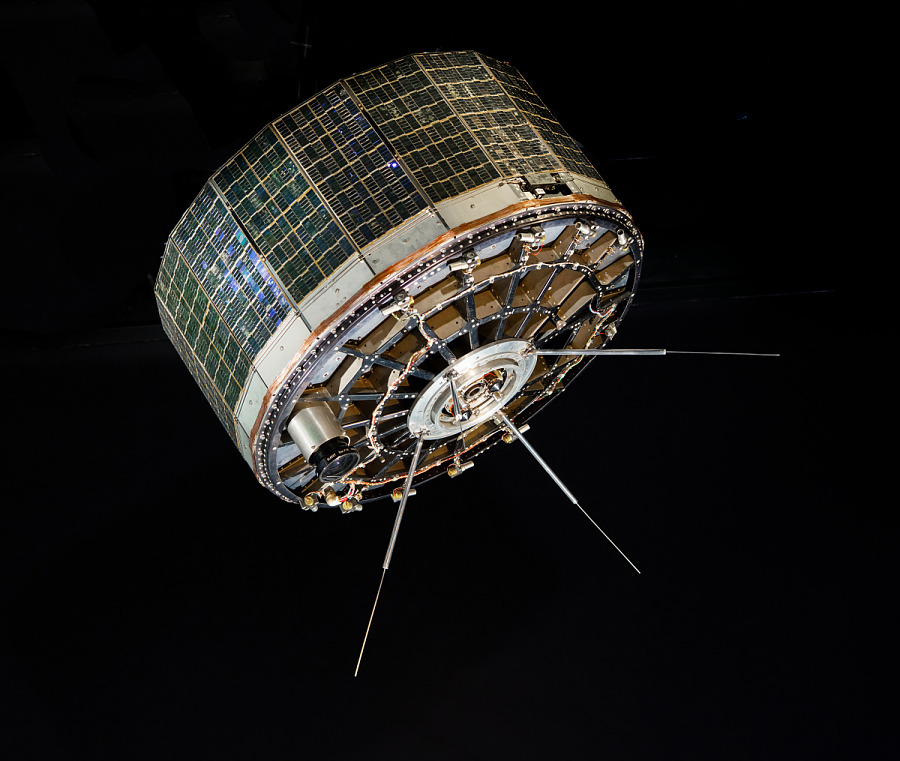
\includegraphics[width=0.35\textwidth]{../resources/tiros.jpg}
    \caption{TIROS műhold}
    \label{fig:tiros}
\end{figure}

\subsection*{Műholdpályák}

A meteorológiai műholdak két fő pályatípuson keringenek: geostacionárius (GEO) és alacsony Föld körüli (LEO) pályán. Utóbbin belül pedig a legelterjedtebb a napszinkron (SSO)
pálya. Ezek a \autoref{fig:geo_leo}-n is láthatóak.

\begin{figure}[H]
    \centering
    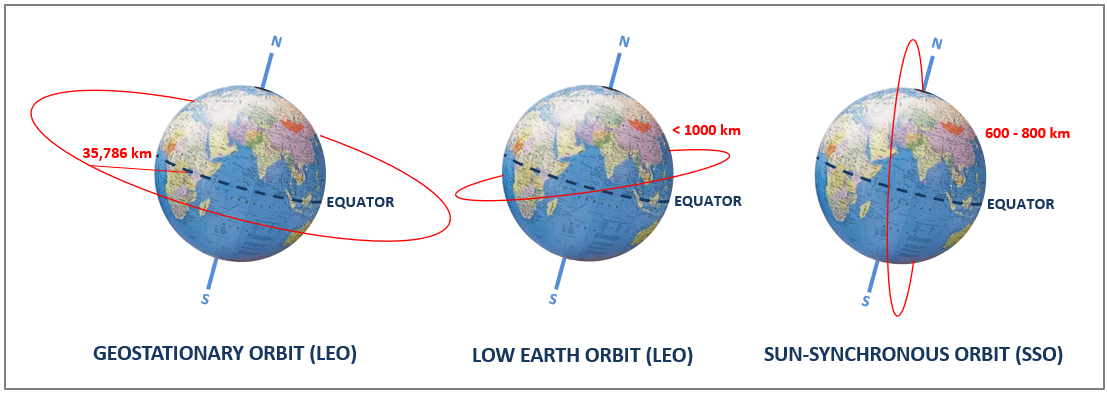
\includegraphics[width=0.75\textwidth]{../resources/orbit-types.png}
    \caption{GEO és LEO pályák összehasonlítása}
    \label{fig:geo_leo}
\end{figure}

\subsubsection*{Geostacionárius pálya (GEO)}
A geoszinkron pályák, olyan pályák melyeknél a keringési idő megegyezik a Föld sziderikus (állócsillagokhoz képes mért) tengelyforgási idejével. A geoszinkron pályák eseténben adott helyi időkor egy ideig minden nap pontosan ugyanazon a földrajzi hely fölött halad.
A geostacionárius pálya a geoszinkron pályák egy speciális esete, amikor is a félnagytengely 42163 km, excentricitás 0, és inklináció 0 fok. Így a Föld felszínéhez képest állandó helyzetben látszik.

A GEO pályán keringő műholdak nagy technikai előnye, hogy nincs szükség antennaforgatóra, egy fix irányba állított antennával is lehet venni és az év csak rövid szakaszában lehet venni.
Hátránya, hogy ebben a nagyobb keringési magasság miatt nagyobb antennanyereség szükséges, valamint ugyanazon mérések kisebb felbontással üzemelnek, mint a LEO pályán.

\subsubsection*{Alacsony Föld körüli pálya (LEO)}

A LEO pályák, olyan pályák melyek magassága 200-2000 km között van. Az itt keringő műholdak keringési ideje 1,5-2 óra között van. Így egy nap alatt többször is megkerülik a Földet. A GEO pályához képest viszonylag kis területet látnak be, de azt sokkal nagyobb felbontásban.
A LEO pályák egy speciális esete a nap-szinkron (SSO) pálya. Ilyenkor a műhold Naphoz viszonyított helyzete állandó, azaz áthaladáskor ugyanabban a helyi időben halad el adott koordináta felett, azonos megvilágítási viszonyok mellett. Mivel a sarkok felett halad el, ezért napjában 2-szer teljesen végigpásztázza a Föld felszínét.
Azonban ilyenkor antennaforgatót kell alkalmazni.

\subsection*{Műholdak vétele}

\subsubsection*{LEO pályás műholdak vétele}

A LEO pályás műholdak vétele VHF (137 MHz), L (1,7 GHz) és X (8 GHz) sávokban történik. A mérési jegyzőkönyv az előbbi kettőt részlétezi.
137 MHz-en alacsony sebességgel analóg képadat továbbítás történik. Ezt alkalmazta a már említett TIROS műholdsorozat is az 1960-as években. Ezek egyszerű és olcsó földiállomásokkal vehetők, azonban az ilyen adóvl felszerelt műholdakat nem tervezik pótolni a jövőben.
Ezzel szemben 1,7 GHz-en digitális adatátivetelt valósítottak meg BPSK vagy QPSK modulációval. Ezek a megoldások nagyobb, parabola antennát és precízebb követést igényelnek.

Egy pályakövető rendszer két fő részből áll: beltéri és kültéri egység.

A beltéri egység áll egy 1,5 m átmérőjű parabololantennából, polarizált patch sugárzóval, egy BPF szűrőbőé és egy kiszajú erősítőből.
A vételi egység folyamatosan meghatározza az azimutot és elevációt ezzel lekövetke a műholdat.
A mérési jegyzőkönyv által ismeretett módszerben egy HackRF SDR veszi a jelet. A digitalizált jelet számítógépen dolgozzuk fel. Erre egy alkalmas nyílt forráskódú program a Sat-Dump.

137 MHz-en egyszerűbb a vételi oldal felépítése. A mérési segédlet egy kételemes Yagi-Uda antennával való vételt ismertet. Ekkor az antenna fixen zenitre van irányítva. Az entenna kimenete ismét egy BPF szűrőre valamint
egy kiszajú erősítőre van kötve. A koaxiális kábel egy RSP1A SDR vevőhöz csatlakozik, aminek a kimenetéből származó FM modulált jelből 2,4 kHz-es vivőjű AM modulált jelet kapunk. A kép kinyerését a WXtoImg program segítségével kapjuk meg.

\subsubsection*{GEO pályás műholdak vétele}
A GEO pályás műholdak esetében is megkülönböztettük a kültéri és beltéri egységet.

\section*{Himawari-9 műhold}

Felhasznált irodalom:\\
Űrtechnológia laboratórium 2 - Laboratóriumi mérési űtmutató\\
Almár - Both - Horváth - Szabó: SH atlasz, Űrtan
\end{document}
